%%%% Paramétrage du TD %%%%
\def\xxactivite{ \ifprof \normalsize{Application 3 -- Corrigé } \else  \ifcolle Colle \else  Application 3\fi \fi} % \normalsize \vspace{-.4cm}
\def\xxauteur{\textsl{Xavier Pessoles}}


\def\xxnumchapitre{Chapitre 1 \vspace{.2cm}}
\def\xxchapitre{\hspace{.12cm} Approche énergétique}

\def\xxcompetences{%
\footnotesize{
\textsl{%
\textbf{Savoirs et compétences :}\\
\vspace{-.2cm}
\begin{itemize}[label=\ding{112},font=\color{ocre}] 
\item Mod2.C18.SF1 : Déterminer l’énergie cinétique d’un solide, ou d’un ensemble de solides, dans son mouvement par rapport à un autre solide.
\item Res1.C1.SF1 : Proposer une démarche permettant la détermination de la loi de mouvement.
%\item Mod1.C5.SF2 : Déterminer la puissance des actions mécaniques extérieures à un solide ou à un ensemble de solides, dans son mouvement rapport à un autre solide.
%\item Mod1.C5.SF3 : Déterminer la puissance des actions mécaniques intérieures à un ensemble de solides.
\end{itemize}}}}

\def\xxtitreexo{Chariot élévateur à bateaux}
\def\xxsourceexo{\hspace{.2cm} \footnotesize{X -- ENS -- PSI -- 2012}}

\def\xxfigures{
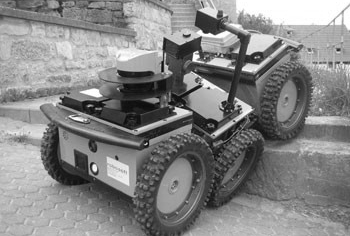
\includegraphics[width=.57\linewidth]{fig_00}
}%figues de la page de garde


\input{\repRel/Style/pagegarde_TD}
\setcounter{numques}{0}

\setlength{\columnseprule}{.1pt}

\pagestyle{fancy}
\thispagestyle{plain}


\vspace{5.2cm}

\def\columnseprulecolor{\color{ocre}}
\setlength{\columnseprule}{0.4pt} 

%%%%%%%%%%%%%%%%%%%%%%%

\setcounter{exo}{0}

\ifprof
%\begin{multicols}{2}
\else
\begin{multicols}{2}
\fi

\subsection*{Présentation}
Le chariot élévateur , objet de cette étude,  permet la manutention de bateaux de \SI{3000}{kg}
à une hauteur de \SI{8}{m}. Il est principalement constitué :
\begin{itemize}
\item du chariot qui assure le déplacement de l’ensemble et apporte la puissance pour la préhension
et le levage ;
\item du tablier, constitué du mât et des fourches, qui permet la préhension et la dépose du bateau.
\end{itemize}

\begin{center}
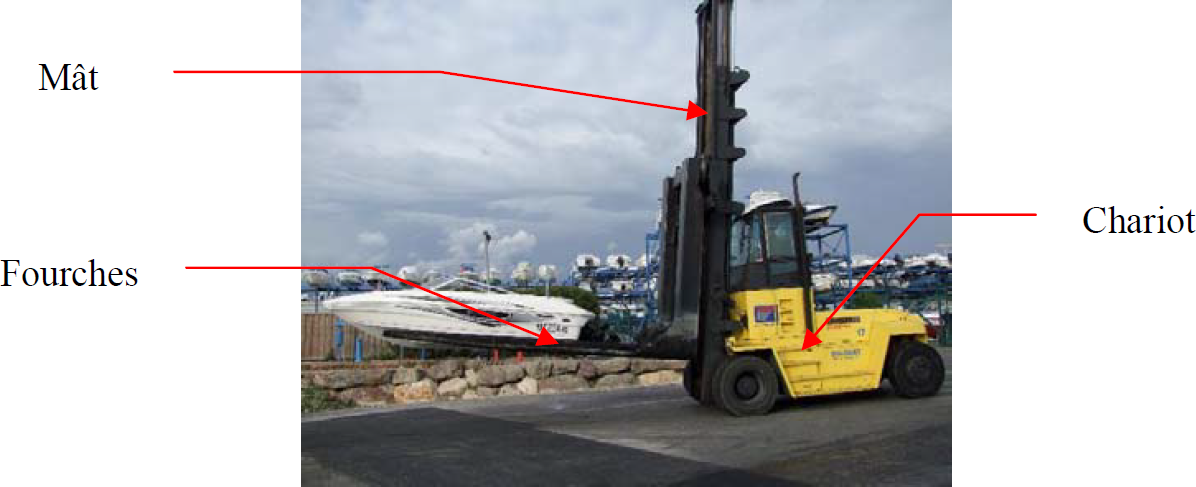
\includegraphics[width=\linewidth]{fig_01a}
\end{center} 



\subsection*{Phase de levage du bateau}
\begin{obj}
Permettre au conducteur de charger et décharger le bateau en toute sécurité : 
\begin{itemize}
\item req 102 : vitesse de levage en charge : \SI{0,33}{m.s^{-1}};
\item req 103 : temps pour atteindre la vitesse de levage en charge : \SI{0,4}{s}.
\end{itemize}
\end{obj}
Dans cette partie, on considère que le chariot est à l’arrêt et que le levage est le seul mouvement actif. Le modèle retenu pour cette étude est le schéma de principe de la suivante. En raison de la symétrie du tablier par rapport à son plan médian vertical, le modèle d’étude peut se ramener à un système comprenant un seul vérin, une seule chaîne et une seule poulie.% L’adaptation des caractéristiques
%cinétiques des différents solides est déjà prise en compte dans les données fournies dans le sujet afin d’assurer la cohérence entre le système réel et la modélisation choisie.
L’actionneur est un vérin hydraulique dont le corps est en liaison encastrement avec le mât inférieur. La tige est solidaire du mât supérieur. Le levage de l’ensemble S=\{T5,T6,T7,T8,T9,T10,T11\} est obtenu à l’aide d’une chaîne présentant un point d’ancrage sur le mât inférieur et un point d’ancrage sur l’ensemble S. Cette chaîne roule sans glisser sur le pignon T12 qui est en liaison pivot par rapport au mât supérieur.
Le bateau étant à l’arrêt en position basse, le conducteur actionne le levage du bateau.
L’effort de poussée fourni par le vérin est $F_V$ (considéré comme constant). 
On note $I_{T12}$ le moment d’inertie de la poulie T12 par rapport à son axe de rotation, $R_{T12}$ son rayon. Sa masse est négligée.
Les masses des différents solides sont rappelées dans le tableau ci-dessous :
\begin{center}
\begin{tabular}{|c|c|}
\hline 
Solide & Masse \\
\hline
Ensemble (S) & $m_S$ \\ \hline
Bateau (B) & $m_B$ \\ \hline
Mât inférieur (T3) & $m_{T3}$ \\ \hline
Mât supérieur (T4) & $m_{T4}$ \\ \hline
Chaîne (C) & négligée \\ \hline
\end{tabular}
\end{center}

Les liaisons sont parfaites. La chaîne est non dissipative. Le repère $\rep{3}$ peut être considéré comme un référentiel galiléen pour les conditions de l’étude. Les axes $\vect{z_{T3}}$ et $\vect{z_{0}}$ sont confondus pour les conditions de l’étude.

\begin{center}
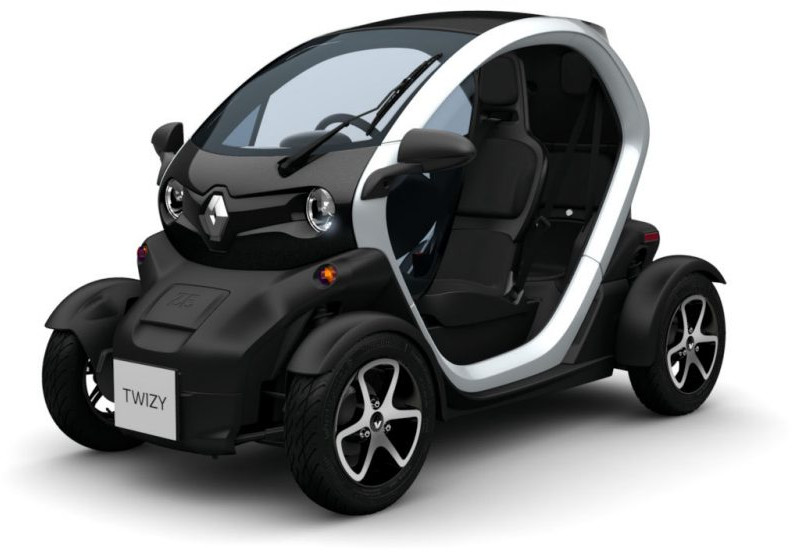
\includegraphics[width=\linewidth]{fig_01}
\end{center}

\question{Déterminer l’accélération galiléenne du bateau en fonction de l’effort fourni par le vérin et des caractéristiques du système. Expliquer qualitativement comment cette valeur peut permettre de valider l'exigence 103.}
\ifprof
\begin{corrige}
\end{corrige}
\else
\fi



\subsection*{Phase de déplacement}
La zone de stockage des bateaux se situe nécessairement à une altitude supérieure à celle du quai de déchargement. Afin d’éviter le glissement du bateau lorsque le chariot descend une pente, un dispositif permet de maintenir les fourches horizontales durant le déplacement. Lors d’une phase de décélération, les fourches sont automatiquement inclinées vers l’arrière pour éviter le glissement du bateau. Ce mouvement, de faible amplitude, est assuré par l’asservissement des vérins d’inclinaison du tablier T1,T2 et T1’, T2’. Ce dispositif présente l’avantage de prendre en charge de manière entièrement automatisée l’un des mouvements du tablier. Le conducteur peut alors charger et mettre à l’eau le bateau sans avoir à gérer manuellement le mouvement d’inclinaison.
La figure suivante permet de définir :
\begin{itemize}
\item l'angle de basculement $\alpha=\angl{z_1}{z_{T3}}$;
\item l'angle de la pente $\delta=\angl{z_0}{z_1}$;
\item l'angle à asservir  $\varphi=\angl{z_0}{z_{T3}}=\alpha+\delta$.
\end{itemize}


\begin{center}
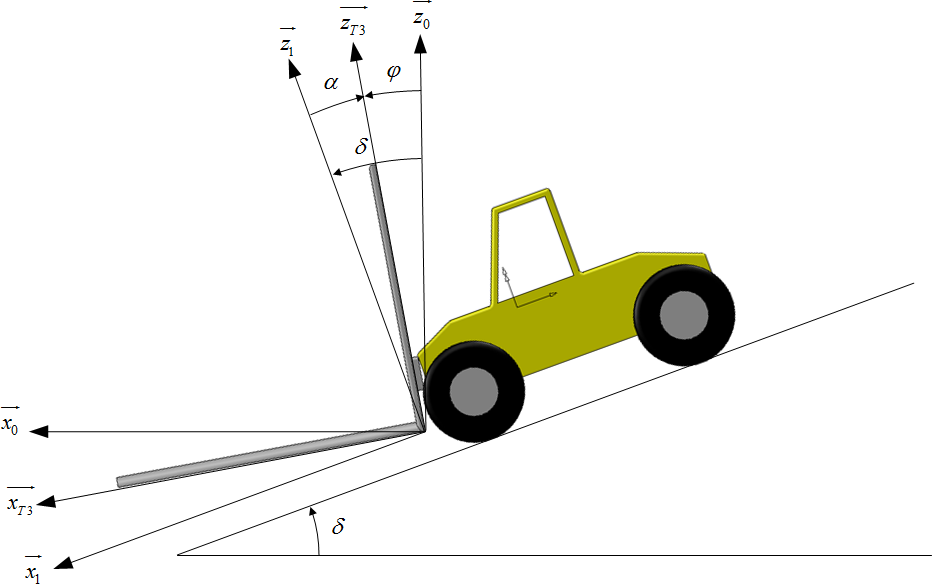
\includegraphics[width=\linewidth]{fig_02}
\end{center}


\question{Quand le chariot circule à vitesse constante, quelle est la valeur de l’angle $\varphi(t)$ qui permet d’assurer le maintien de l’horizontalité des fourches ? Justifier.}
\ifprof
\begin{corrige}
\end{corrige}
\else
\fi



Nous considérons dans cette partie que le seul mouvement actif est le basculement.
L’objectif est d’obtenir un modèle dynamique du mécanisme de basculement à partir de la modélisation plane proposée sur la figure suivante.


\begin{center}
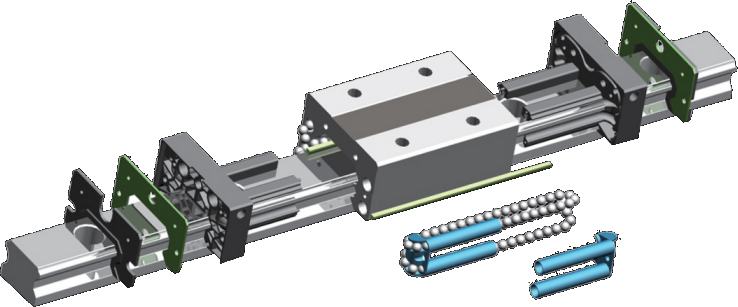
\includegraphics[width=\linewidth]{fig_03}
\end{center}

Les solides pris en compte pour l’étude sont :
\begin{itemize}
\item l'ensemble $S_2$=\{ T3, T4, T5, T6, T7, T8, T9, T10, T11, B\} en liaison pivot d'axe $\axe{O_1}{y_0}$ par rapport au chariot 1 de centre de gravité $G_{S_2}$. Le moment d’inertie de l’ensemble $S_2$ par rapport à l’axe sera noté $J_{S2}$ et sa masse $m_{S2}$. La liaison pivot entre l’ensemble $S_2$ et le chariot (bâti) génère un couple résistant $\vect{C_{\mu}}=-\mu\dot{\alpha}\vect{y_0}$ et $\vect{O_1O_{G_{S2}}}=x_{G_{S2}} \vect{x_{T3}}+z_{G_{S2}} \vect{z_{T3}}$; 
\item un vérin équivalent $V=\left\{ T1,T2\right\}$ dont le corps est en liaison pivot d’axe $\axe{A_1}{y_0}$ par rapport au chariot (bâti) et la tige en liaison pivot d’axe $\axe{B_1}{y_0}$ par rapport à l’ensemble $S_2$. La masse et l’inertie du vérin sont négligées. Le vérin développe un effort au cours du mouvement qui sera noté $\vect{F_V} = p(t) S \vect{z_{T2}}$ où $p(t)$ est la différence de pression entre les deux chambres du vérin.
\end{itemize}


On pose $\vect{A_1B_1} = \left( \lambda_0+\lambda\right)\vect{z_{T2}}$. Le paramétrage est tel que si $\alpha=0$ alors $\lambda=0$.

%
%
%Une simulation a permis de tracer la courbe qui donne $\alpha(t)$ en fonction de $\lambda(t)$ sur la plage de variation de $\alpha(t)$ qui correspond au mouvement de basculement. L’analyse de cette courbe nous permet d’approximer une relation linéaire entre $\alpha(t)$ et $\lambda(t)$ de la forme $\alpha(t)=k\lambda(t)$ où $k$ est une constante.


\question{En appliquant le théorème de l’énergie-puissance et en admettant que l’angle $\alpha$ est petit, montrer que $\alpha(t)$ et $p(t)$ sont liés par l’équation différentielle suivante :  $J_{\text{eq}}\ddot{\alpha}(t) + \mu \dot{\alpha}(t) =\dfrac{Sp(t)}{k}+m_{S_2}g x_{G_{S_2}}$. Exprimer $J_{\text{eq}}$.}
\ifprof
\begin{corrige}
\end{corrige}
\else
\fi

\ifprof
%\end{multicols}%
\else
\end{multicols}%
\fi

